\documentclass{beamer}
% \mode<presentation>
\setbeamertemplate{navigation symbols}{}
\let\tempone\itemize
\let\temptwo\enditemize
\renewenvironment{itemize}{\tempone\addtolength{\itemsep}{0.5\baselineskip}}{\temptwo}
\usepackage{beamerthemeshadow}
\usepackage{tikz}
\usepackage{bbm}
\usepackage{hyperref}
\usepackage{natbib}
\usepackage{pgffor}
\usepackage{booktabs}
\usepackage{graphicx}
\usepackage{amssymb}
\usepackage{tabularx}
\usepackage{tikz,etoolbox}
\usepackage{tikz,amsmath,siunitx}
\usetikzlibrary{arrows,snakes,backgrounds,patterns,matrix,shapes,fit,calc,shadows,plotmarks}
\newcommand{\softmax}{\mathrm{softmax}}
\usepackage[normalem]{ulem}
\newcommand\tst{% thick strike through  %% from http://tex.stackexchange.com/questions/134088/mis-alignment-of-columns-in-tabular-environment-when-using-ulem-and-beamer
  \bgroup%
  \markoverwith{\textcolor{red}{\rule[1.1ex]{1pt}{0.8pt}}}%
  \ULon%
}

\usepackage{subcaption}
\usepackage[absolute,overlay]{textpos}
\usepackage{pgf}
\usepackage{latexsym}
\usepackage{amsfonts}
\usepackage{amssymb}
\usepackage{amsthm}
\usepackage{algorithm}
\usepackage{amsmath}
\usepackage{tabularx}
\usepackage{xcolor}
\usepackage[absolute,overlay]{textpos}
\usetikzlibrary{shapes,arrows,positioning,automata,positioning,spy,matrix,scopes,chains}
\newcommand{\digs}[2]{\hphantom{999}\llap{#1}\,+\,\hphantom{999}\llap{#2}}
\setbeamersize{text margin left=6mm}
\setbeamersize{text margin right=6mm}
\renewcommand{\insertnavigation}[1]{}
\setbeamertemplate{headline}{}
\setbeamertemplate{footline}{}
\usefonttheme{professionalfonts}
\setbeamercovered{transparent}
\mode<presentation>
\linespread{1.25}
\DeclareMathOperator{\Tr}{Tr} 

\usepackage{color}
\usepackage{multirow}
\usepackage{rotating}
\usepackage[all,dvips]{xy}
\usepackage{colortbl}
\usepackage{graphicx}
\usepackage{verbatim}
\usepackage{framed}
\usepackage{natbib}
\usepackage[labelformat=empty]{caption}
\newcommand{\air}{\vspace{0.25cm}}
\newcommand{\mair}{\vspace{-0.25cm}}

\setbeamertemplate{navigation symbols}{}%remove navigation symbols
\renewcommand{\rmdefault}{crm}
\newcommand{\lnbrack}{{\normalfont [}}
\newcommand{\rnbrack}{{\normalfont ]}\thinspace}
\newcommand{\lbbrack}{\textcolor{red}{\textbf{[}}}
\newcommand{\rbbrack}{\textcolor{red}{\textbf{]}}\thinspace}
\definecolor{vermillion}{RGB}{213,94,0}
\newcommand{\given}{\,|\,}
\definecolor{orange}{RGB}{230,159,0}
\definecolor{skyblue}{RGB}{86,180,233}
\definecolor{bluegreen}{RGB}{90,143,41}
% \definecolor{bluegreen}{RGB}{0,158,115}
\definecolor{myyellow}{RGB}{240,228,66} % i dunno if this is the same as standard yellow
\definecolor{myblue}{RGB}{0,114,178}
\definecolor{vermillion}{RGB}{213,94,0}
\definecolor{redpurple}{RGB}{204,121,167}
\definecolor{lightgrey}{RGB}{234,234,234}

\newcommand{\clust}{\ensuremath{\mathrm{clust}}}
\newcommand{\loc}{\ensuremath{\mathrm{loc}}}
\newcommand{\nicein}{\ensuremath{\,{\in}\,}}
\newcommand{\niceq}{\ensuremath{\,{=}\,}}
\newcommand{\uc}{\ensuremath{\mathrm{c}}}
\newcommand{\hc}{\boldh_{\uc}}
\newcommand{\cb}{\boldb_{\mathrm{\uc}}}
\newcommand{\cW}{\boldW_{\mathrm{\uc}}}

\newcommand{\ha}{\boldh_{\ua}}
\newcommand{\hp}{\boldh_{\up}}
% \newcommand{\hc}{\boldh_{\mathrm{c}}}


\def\kargmax{\operatornamewithlimits{K-arg\,max}}
%\DeclareMathOperator{\topK}{topK}
\def\topK{\operatornamewithlimits{topK}}
\DeclareMathOperator{\suk}{succ}
\newcommand{\longpfx}[1]{\ensuremath{w_1 \cdots w_{#1}}}
\newcommand{\longgoldpfx}[1]{\ensuremath{y_1 \cdots y_{#1}}}
\newcommand{\pfx}[1]{\ensuremath{w_{1:{#1}}}}
\newcommand{\goldpfx}[1]{\ensuremath{y_{1:{#1}}}}
\newcommand{\beampred}[2]{\ensuremath{\hat{y}_{1:{#1}}^{({#2})}}}
\newcommand{\boldx}{\mathbf{x}}

\usetikzlibrary{positioning}
% \setbeamerfont{alerted text}{series=\bfseries}
% \setbeamerfont{structure}{series=\bfseries}
% Needed for diakgrams.
\def\im#1#2{
  \node(#1) [scale=#2]{\pgfbox[center,top]{\pgfuseimage{#1}}
};}
% \input{pictures_header}


\title[Seq2seq]{CS182 Guest Lecture: \\ Deep Learning for Text Generation}


\author[Alexander Rush]{Alexander Rush  (@harvardnlp) \\  
{\scriptsize  (with  Yoon Kim, Sam Wiseman, Hendrik Strobelt, Yuntian Deng, Allen Schmaltz) } \\
% \url{http://www.github.com/harvardnlp/seq2seq-talk/}
} 

\institute[Harvard SEAS]{ \\
  \begin{center}
    
\includegraphics[width=1.3cm]{seas}
  \end{center}

}
\date{}
% \usetheme{Madrid}

\newcommand{\enc}{\mathrm{src}}
\newcommand{\xvec}{\mathbf{x}}
\newcommand{\yvec}{\mathbf{y}}
\newcommand{\wvec}{\mathbf{w}}
\newcommand{\cvec}{\mathbf{c}}
\newcommand{\zvec}{\mathbf{z}}
% \newcommand{\mcY}{\mathcal{Y}}
% \newcommand{\mcV}{\mathcal{V}}
\newcommand{\context}{\mathbf{w}_{\mathrm{c}}}
\newcommand{\embcontext}{\mathbf{\tilde{w}}_{\mathrm{c}}}
\newcommand{\inpcontext}{\mathbf{\tilde{x}}}
\newcommand{\start}{\mathbf{\tilde{y}}_{\mathrm{c0}}}
\newcommand{\End}{\mathrm{\texttt{</s>}}}

\newcommand{\Uvec}{\mathbf{U}}
\newcommand{\Evec}{\mathbf{E}}
\newcommand{\Gvec}{\mathbf{G}}
\newcommand{\Fvec}{\mathbf{F}}
\newcommand{\Pvec}{\mathbf{P}}
\newcommand{\pvec}{\mathbf{p}}
\newcommand{\Qvec}{\mathbf{Q}}
\newcommand{\Vvec}{\mathbf{V}}
\newcommand{\Wvec}{\mathbf{W}}
\newcommand{\hvec}{\mathbf{h}}
% \newcommand{\reals}{\mathbb{R}}

\newcommand{\Cite}[1]{{\footnotesize \citep{#1}}}
\newcommand{\TT}[1]{{\footnotesize\tt{#1}}}
\newcommand{\boldw}{\boldsymbol{w}}
\newcommand{\boldu}{\boldsymbol{u}}
\newcommand{\boldv}{\boldsymbol{v}}
\newcommand{\boldb}{\mathbf{b}}
\newcommand{\boldW}{\mathbf{W}}
\newcommand{\boldh}{\boldsymbol{h}}
\newcommand{\boldg}{\boldsymbol{g}}
\newcommand{\ua}{\ensuremath{\mathrm{a}}}
\newcommand{\up}{\ensuremath{\mathrm{p}}}
%\newcommand{\bphi}{\ensuremath{\mathbf{\phi}}}
\newcommand{\bphi}{\boldsymbol{\phi}}
\newcommand{\btheta}{\boldsymbol{\theta}}
\newcommand{\mcY}{\mathcal{Y}}
\newcommand{\mcX}{\mathcal{X}}
\newcommand{\mcC}{\mathcal{C}}
\newcommand{\mcA}{\mathcal{A}}
\newcommand{\mcV}{\mathcal{V}}
\newcommand{\trans}{\ensuremath{\mathsf{T}}}
\def\argmin{\operatornamewithlimits{arg\,min}}
\def\argmax{\operatornamewithlimits{arg\,max}}
\newcommand{\reals}{\ensuremath{\mathbb{R}}}

\newcommand{\aphi}{\boldsymbol{\phi}_{\mathrm{a}}}
\newcommand{\pwphi}{\boldsymbol{\phi}_{\mathrm{p}}}
\newcommand{\squigaphi}{\widetilde{\boldsymbol{\phi}}_{\mathrm{a}}}
\newcommand{\squigpwphi}{\widetilde{\boldsymbol{\phi}}_{\mathrm{p}}}

\newcommand{\aW}{\boldW_{\mathrm{\ua}}}
\newcommand{\pW}{\boldW_{\mathrm{\up}}}

\newcommand{\ab}{\boldb_{\mathrm{\ua}}}
\newcommand{\pb}{\boldb_{\mathrm{\up}}}

\newcommand{\Da}{d_{\mathrm{a}}}
\newcommand{\Dp}{d_{\mathrm{p}}}

% \newcommand{\ha}{\boldh_{\ua}}
% \newcommand{\hp}{\boldh_{\up}}

\newcommand{\ourmodel}{This work}
\newcommand{\zro}{{\color{white}0}}


\def\argmax{\operatornamewithlimits{arg\,max}}
\def\kargmax{\operatornamewithlimits{K-arg\,max}}

\begin{document}

\begin{frame}
  \titlepage
\end{frame}

\begin{frame}
  \begin{center}
    \textbf{Language Models}
  \end{center}
\end{frame}

\begin{frame}
  \only<1>{
  \begin{center}
    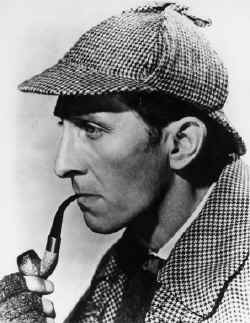
\includegraphics[width=3cm]{holmes}
  \end{center}
}
\only<2>{
  \begin{center}
    \begin{tikzpicture}[spy using outlines={circle, magnification=20,
        size=3cm, connect spies}]
      \node {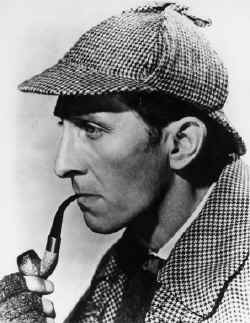
\includegraphics[width=3cm]{holmes}}; 
      \spy [cyan] on
      (0.0,0.3) in node [left] at (5.4,-1.15);
    \end{tikzpicture}
  \end{center}
}
  \begin{quote}
    It is a capital mistake to theorize before one has
    data. Insensibly one begins to twist facts to suit theories,
    instead of theories to suit facts. -Sherlock Holmes, A Scandal in Bohemia
  \end{quote}


\end{frame}

\begin{frame}

  \begin{center}
    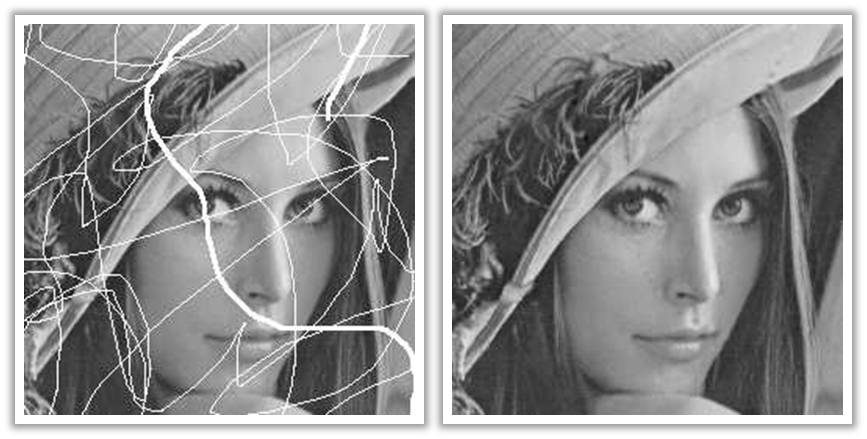
\includegraphics[width=6cm]{lena}
  \end{center}

  \air
  \only<1> {
    \begin{quote}
    It is a capital mistake to theorize before one has \_\_\_\_\_\_ $\ldots$ 
    \end{quote}
  }
  \only<2> {
    \begin{quote}
      108 938 285 28 184 29 593 219 58 772 \_\_\_\_\_\_ $\ldots$ 
    \end{quote}    
  }
\end{frame}



\begin{frame}
  \begin{center}
    \structure{Language Modeling Task}
  \end{center}
  Given a sequence of text give a probability distribution 
  over the next word. 

\air

  The Shannon game. Estimate the probability of the next letter/word
  given the previous.

  \begin{quote}
    THE ROOM WAS NOT VERY LIGHT A SMALL OBLONG READING LAMP ON THE
    DESK SHED GLOW ON POLISHED \_\_\_\
  \end{quote}


\end{frame}


\begin{frame}
  \begin{center}
    \structure{Shannon (1948) \textit{Mathematical Model of Communication}}
  \end{center}
\air
  
\begin{quote}  
  We may consider a discrete source, therefore,
to be represented by a stochastic process. Conversely, any stochastic
process which produces a discrete sequence of symbols chosen from a finite
set may be considered a discrete source. This will include such cases as:

1. Natural written languages such as English, German, Chinese.
...
\end{quote}
\end{frame}

\begin{frame}[allowframebreaks]
  \begin{center}
    \structure{Shannon's Babblers}
  \end{center}
  \begin{quote}
   
  4. Third-order approximation (trigram structure as in English).

IN NO 1ST LAT WHEY CRATICT FROURE BIRS GROCID
PONDENOME OF DEMONSTURES OF THE REPTAGIN IS
REGOACTIONA OF CRE
  \end{quote}

  \begin{quote}
5. First-Order Word Approximation. Rather than continue with tetragram,
... , II-gram structure it is easier and better to jump at this
point to word units. Here words are chosen independently but with
their appropriate frequencies.

REPRESENTING AND SPEEDILY IS AN GOOD APT OR
COME CAN DIFFERENT NATURAL HERE HE THE A IN
CAME THE TO OF TO EXPERT GRAY COME TO FURNISHES
THE LINE MESSAGE HAD BE THESE.

  \end{quote}

  \begin{quote}
    6. Second-Order Word Approximation. The word transition probabilities
are correct but no further structure is included.

THE HEAD AND IN FRONTAL ATTACK ON AN ENGLISH
'RITER THAT THE CHARACTER OF THIS POINT IS
THEREFORE ANOTHER METHOD FOR THE LETTERS
THAT THE TIME OF WHO EVER TOLD THE PROBLEM
FOR AN UNEXPECTED

The resemblance to ordinary English text increases quite noticeably at
each of the above steps.

  \end{quote}
\end{frame}

\begin{frame}
  \begin{center}
    \textbf{Simple Language Models}
  \end{center}
\end{frame}


\begin{frame}

Goal: Estimate Markov model 
\[ p(w_{t} | w_{1}, \ldots, w_{t-1}) \approx p(w_{t} | w_{t-n}, \ldots w_{t-1})\] 

Ingredients: 

\begin{itemize}
\item 1 Corpus (e.g. the entire web)

\end{itemize}

Steps:

\begin{itemize}
\item (1) Collect words, (2) Count up n-grams, (3) Divide$^*$
  \begin{eqnarray*} 
    p(w_{t+1} | w_{t-n+1}, \ldots w_{t}) &=& \frac{\#( w_{t-n+1}, \ldots, w_{t+1}) }{\#( w_{t-n+1}, \ldots, w_{t})} \\
    &=&  \frac{\#(\mathrm{theorize\ before\ one\ has\ data})}{\#(\mathrm{theorize\ before\ one\ has})}
    \end{eqnarray*}
\end{itemize}
\end{frame}

\begin{frame}
  \begin{center}
    \alert{Google 1T}

  \end{center}
  \begin{table}
    \centering
  \begin{tabular}{ll}
    \toprule
    Number of token  &1,024,908,267,229 \\
    Number of sentences & 95,119,665,584 \\
    Size compressed (counts only) & 24 GB \\  
    \midrule
    Number of unigrams & 13,588,391 \\
    Number of bigrams & 314,843,401 \\ 
    Number of trigrams & 977,069,902 \\ 
    Number of fourgrams & 1,313,818,354 \\
    Number of fivegrams&  1,176,470,663 \\
    \bottomrule
  \end{tabular}
  \end{table}


\end{frame}

\begin{frame}
  \textbf{Zipf' Law (1935,1949):}
  \begin{quote}
    The frequency of any word is inversely proportional to its rank in the frequency table.
  \end{quote}


     \begin{center}
       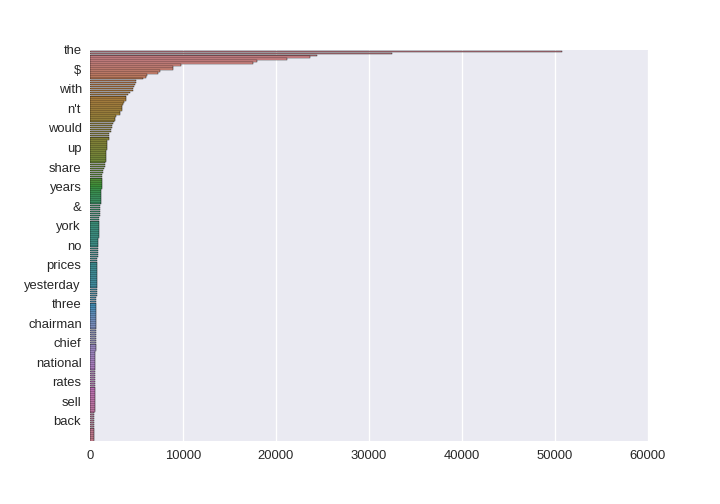
\includegraphics[width=0.8\textwidth]{zipf}         
     \end{center}
\end{frame}


\begin{frame}
  \begin{center}
    \textbf{Neural Networks}
  \end{center}
\end{frame}

\begin{frame}
  \begin{center}
    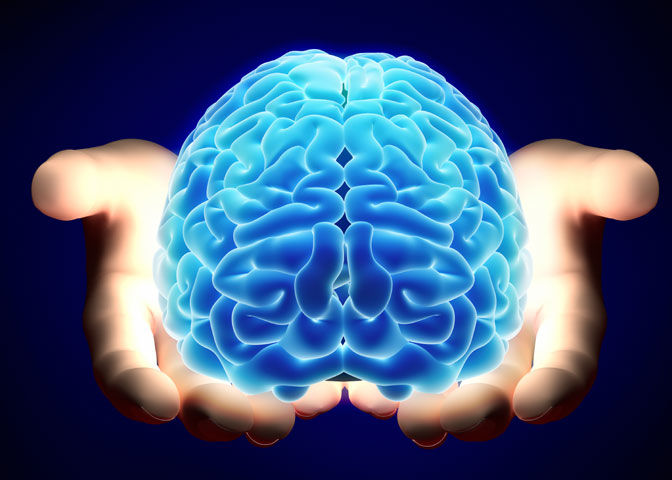
\includegraphics[width=5cm]{brain}
  \end{center}
\end{frame}

\begin{frame}
  A \structure{neural network} is a \alert{function approximator} (no more, no less). 

  
  \begin{itemize}
  \item  $NN(\boldx; \theta)$; a learned function from $\boldx$ with parameters $\theta$.
  \end{itemize}
% \end{frame}

  \pause
% \begin{frame}{Neural Network}
  One-layer of a network architecture.

  \[NN_{MLP1}(\boldx) =  \boldW^2 \sigma(\boldW^1 \boldx + \boldb^1) + \boldb^2\]
  \begin{itemize}
  \item $\boldx$; input

  \item $\boldW, \boldb$; parameters
  % \item $\boldW^1 \in \reals^{\din \times \dhid}, \boldb^1 \in \reals^{1 \times \dhid}$; first affine transformation
  % \item $\boldW^2 \in \reals^{\dhid \times \dout}, \boldb^2 \in \reals^{1 \times \dout}$; second affine transformation
  \item $\sigma$ is \textit{non-linearity} 
  % \item $g(\boldx\boldW^1 + \boldb^1)$ is the \textit{hidden layer}
  \end{itemize}
  \begin{figure}
    \centering
    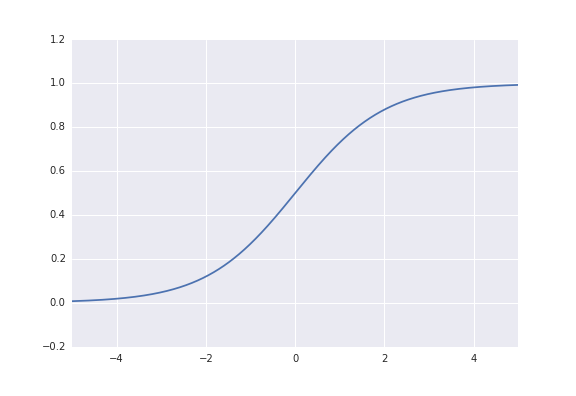
\includegraphics[width=5cm]{sigmoid}     
  \end{figure}

\end{frame}

% \begin{frame}
%   Logistic sigmoid function:
%   \[\sigma(t) = \frac{1}{1 + \exp(-t)} \]
%   \begin{figure}
%     \centering
%     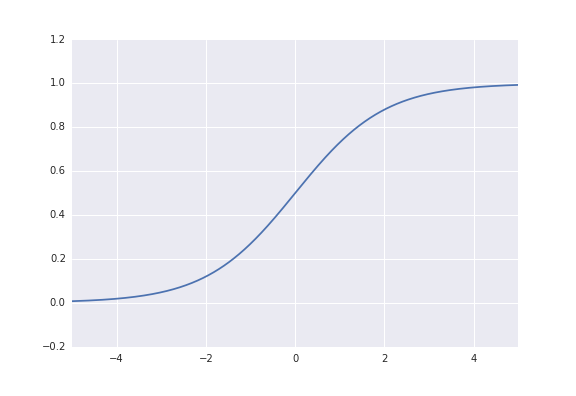
\includegraphics[width=5cm]{sigmoid}     
%   \end{figure}

%   \begin{itemize}
%   \item $\sigma((\boldW^1 \boldx + \boldb^1)_i)$
%   \end{itemize}
% \end{frame}



\begin{frame}
  \begin{center}


  \begin{tikzpicture}
    \node(aa)[draw, circle]{$x_1$};
    \node(ab)[below of =  aa, draw, circle]{$x_2$};
    \node(ac)[below of = ab, draw,circle]{$x_3$};
    \node(ad)[below of = ac]{$\vdots$};
    \node(ae)[below of =  ad, draw, circle]{$x_{\din}$};


    \node(ba)[xshift= 2cm, yshift=-0.5cm, right of = aa, draw, circle]{$h_1$};
    \node(bb)[below of =  ba, draw, circle]{$h_2$};
    \node(bc)[below of = bb]{$\vdots$};

    \node(bd)[below of =  bc, draw, circle]{$h_{\dhid}$};

    \path[draw] (aa) -- (ba);
    \path[draw] (aa) -- (bb);
    \path[draw] (aa) -- (bd);

    \path[draw] (ab) -- (ba);
    \path[draw] (ab) -- (bb);
    \path[draw] (ab) -- (bd);

    \path[draw] (ac) -- (ba);
    \path[draw] (ac) -- (bb);
    \path[draw] (ac) -- (bd);

    \path[draw] (ae) -- (ba);
    \path[draw] (ae) -- (bb);
    \path[draw] (ae) -- (bd);


    \node(ca)[xshift= 2cm, yshift=0.5cm, right of = ba, draw, circle]{$z_1$};
    \node(cb)[below of =  ca, draw, circle]{$z_2$};
    \node(cc)[below of =  cb, draw, circle]{$z_3$};
    \node(cd)[below of = cc]{$\vdots$};
    \node(ce)[below of =  cd, draw, circle]{$z_{\dout}$};


    \path[draw] (ba) -- (ca);
    \path[draw] (ba) -- (cb);
    \path[draw] (ba) -- (cc);
    \path[draw] (ba) -- (ce);

    \path[draw] (bb) -- (ca);
    \path[draw] (bb) -- (cb);
    \path[draw] (bb) -- (cc);
    \path[draw] (bb) -- (ce);

    \path[draw] (bd) -- (ca);
    \path[draw] (bd) -- (cb);
    \path[draw] (bd) -- (cc);
    \path[draw] (bd) -- (ce);


  \end{tikzpicture}
  \end{center}
\end{frame}

\begin{frame}
  \begin{center}
    \textbf{Neural Networks for Language}
  \end{center}
  
  \begin{itemize}
  \item $\boldx$; previous words 
  \item $NN(\boldx)$; score for next word  
  \end{itemize}
  \[NN_{MLP1}(\boldx) =  \boldW^2 \sigma(\boldW^1 \boldx + \boldb^1) + \boldb^2\]

  \begin{center}
    \begin{tikzpicture}
    \node(aa)[draw, circle]{$x_1$};
    \node(ab)[below of =  aa, draw, circle]{$x_2$};
    \node(ac)[below of = ab, draw,circle]{$x_3$};
    \node(ad)[below of = ac]{$\vdots$};
    \node(ae)[below of =  ad, draw, circle]{$x_{\din}$};


    \node(ba)[xshift= 2cm, yshift=-0.5cm, right of = aa, draw, circle]{$h_1$};
    \node(bb)[below of =  ba, draw, circle]{$h_2$};
    \node(bc)[below of = bb]{$\vdots$};

    \node(bd)[below of =  bc, draw, circle]{$h_{\dhid}$};

    \path[draw] (aa) -- (ba);
    \path[draw] (aa) -- (bb);
    \path[draw] (aa) -- (bd);

    \path[draw] (ab) -- (ba);
    \path[draw] (ab) -- (bb);
    \path[draw] (ab) -- (bd);

    \path[draw] (ac) -- (ba);
    \path[draw] (ac) -- (bb);
    \path[draw] (ac) -- (bd);

    \path[draw] (ae) -- (ba);
    \path[draw] (ae) -- (bb);
    \path[draw] (ae) -- (bd);


    \node(ca)[xshift= 2cm, yshift=0.5cm, right of = ba, draw]{word 1};
    \node(cb)[below of =  ca, draw]{word 2};
    \node(cc)[below of =  cb, draw]{word 3};
    \node(cd)[below of = cc]{$\vdots$};
    \node(ce)[below of =  cd, draw]{word n};


    \path[draw] (ba) -- (ca);
    \path[draw] (ba) -- (cb);
    \path[draw] (ba) -- (cc);
    \path[draw] (ba) -- (ce);

    \path[draw] (bb) -- (ca);
    \path[draw] (bb) -- (cb);
    \path[draw] (bb) -- (cc);
    \path[draw] (bb) -- (ce);

    \path[draw] (bd) -- (ca);
    \path[draw] (bd) -- (cb);
    \path[draw] (bd) -- (cc);
    \path[draw] (bd) -- (ce);
  \end{tikzpicture}
\end{center}
\end{frame}



\begin{frame}
  Example:
  
  \begin{itemize}
  \item Consider a language with two words: the, red, and dog. 
  \item We would like the following sentences to be valid: the red dog, the dog red, dog red red, red the dog.

  \item Can you design a neural network to do this?

  \end{itemize}

\end{frame}

\begin{frame}
  \begin{center}
    How does it learn to do this?
  \end{center}

  \begin{itemize}
  \item Very short answer: hill climbing.
    \air 
  \item Backpropagation. Compute gradient, update $\theta$ 
  \end{itemize}
  \begin{center}
    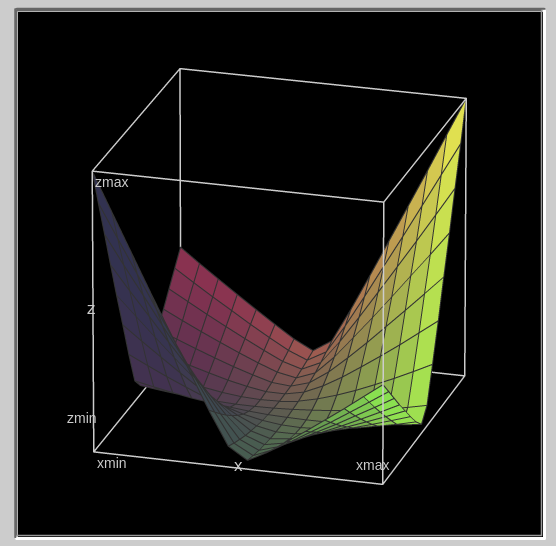
\includegraphics[width=5cm]{logbilinear}
  \end{center}
  
\end{frame}

\begin{frame}
  \begin{center}
    \textbf{Neural Network Language Models}
  \end{center}
\end{frame}


% \begin{frame}
%     \begin{center}
%     \textbf{This Talk: Neural Networks For Language}
%   \end{center}
% \end{frame}


\begin{frame}
  \begin{center}
    \alert{Seq2Seq Neural Network Toolbox}
    \air 
  \end{center}
  \begin{center}
    \begin{tabular}{cclll}
      \structure{Embeddings} & & sparse features &$\Rightarrow$& dense features \\\\
      \structure{RNNs} & & feature sequences & $\Rightarrow$ &dense features \\\\
      \structure{Softmax} & & dense features & $\Rightarrow$ & discrete predictions \\
    \end{tabular}
  \end{center}
\end{frame}

\begin{frame}
  \begin{center}
    \begin{tabular}{cclll}
      \structure{Embeddings} & & sparse features & $\Rightarrow$ & dense features \\\\
    \end{tabular}
  \end{center}

  \begin{center}
    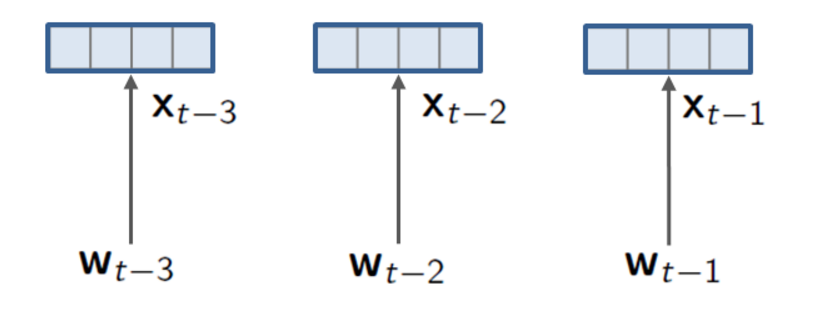
\includegraphics[width=7cm]{emb}
  \end{center}
\end{frame}

\begin{frame}
  \begin{center}
    \includegraphics[height=0.9\textheight]{graph}

    \href[pdfnewwindow=true]{http://harvardnlp.github.io/seq2seq-talk/web/wordvecs.html}{[Words Vectors]}
   \end{center}
\end{frame}


\begin{frame}
  \begin{center}
    \begin{tabular}{cclll}
      \structure{RNNs/LSTMs} & & feature sequences & $\Rightarrow$ &dense features \\\\
    \end{tabular}
  \end{center}


  \begin{center}
    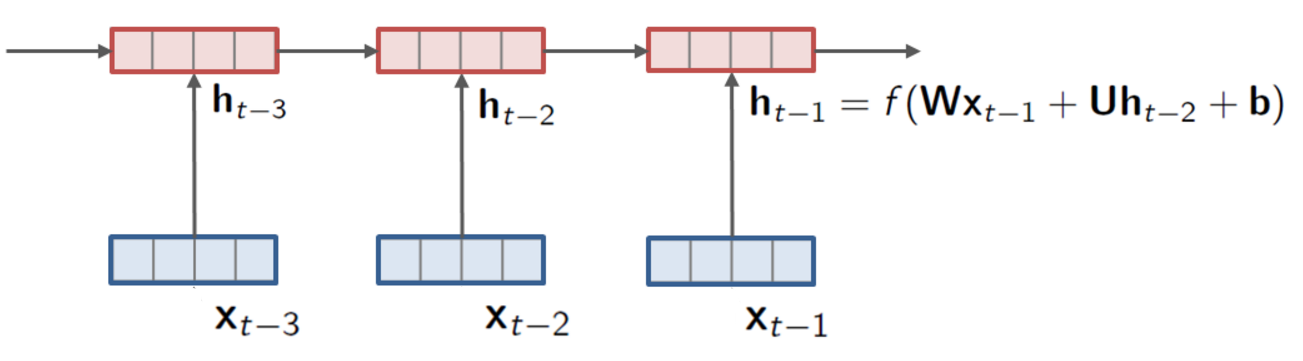
\includegraphics[width=11cm]{rnn}
  \end{center}  
\end{frame}



\begin{frame}
  \begin{center}
    \begin{tabular}{cclll}
      \structure{LM/Softmax} & & dense features & $\Rightarrow$ & discrete predictions \\
    \end{tabular}
    \air 

    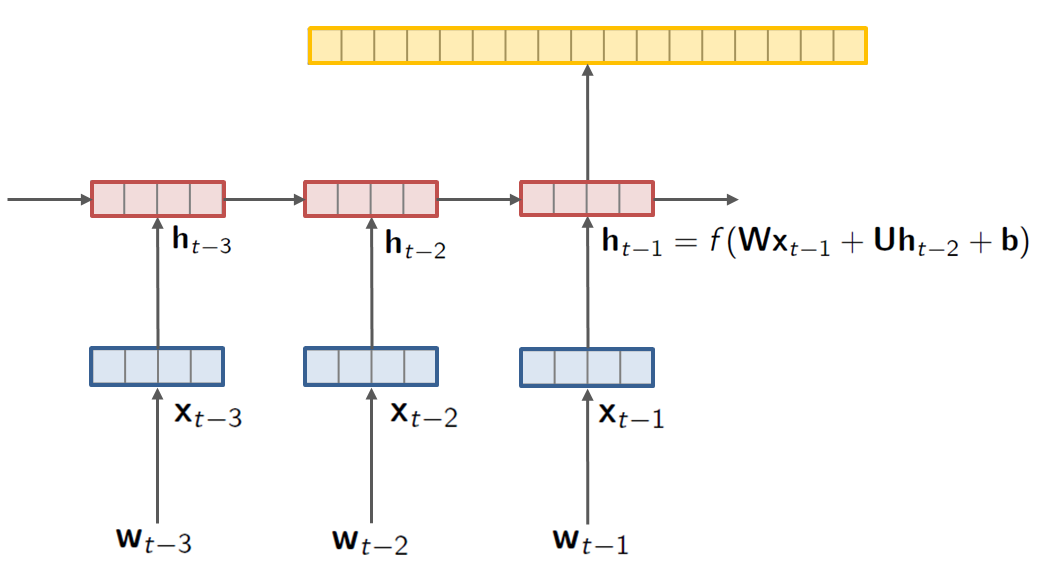
\includegraphics[width=0.8\textwidth]{rnnlm5}
  \end{center}
  \[ p(w_t | w_1, \ldots, w_{t-1}; \theta) = \text{softmax}(\mathbf{W}_{out} \mathbf{h}_{t-1} + \mathbf{b}_{out}) \] 

  \[ p(w_{1:T} ) = \prod_{t} p(w_t | w_1, \ldots, w_{t-1}) \] 
    % \caption{Xu et al (2015)}  
\end{frame}

\begin{frame}
  \begin{center}
    \structure{Contextual Language Model / ``seq2seq''}
  \end{center}
    \air 
   
    \begin{center}
      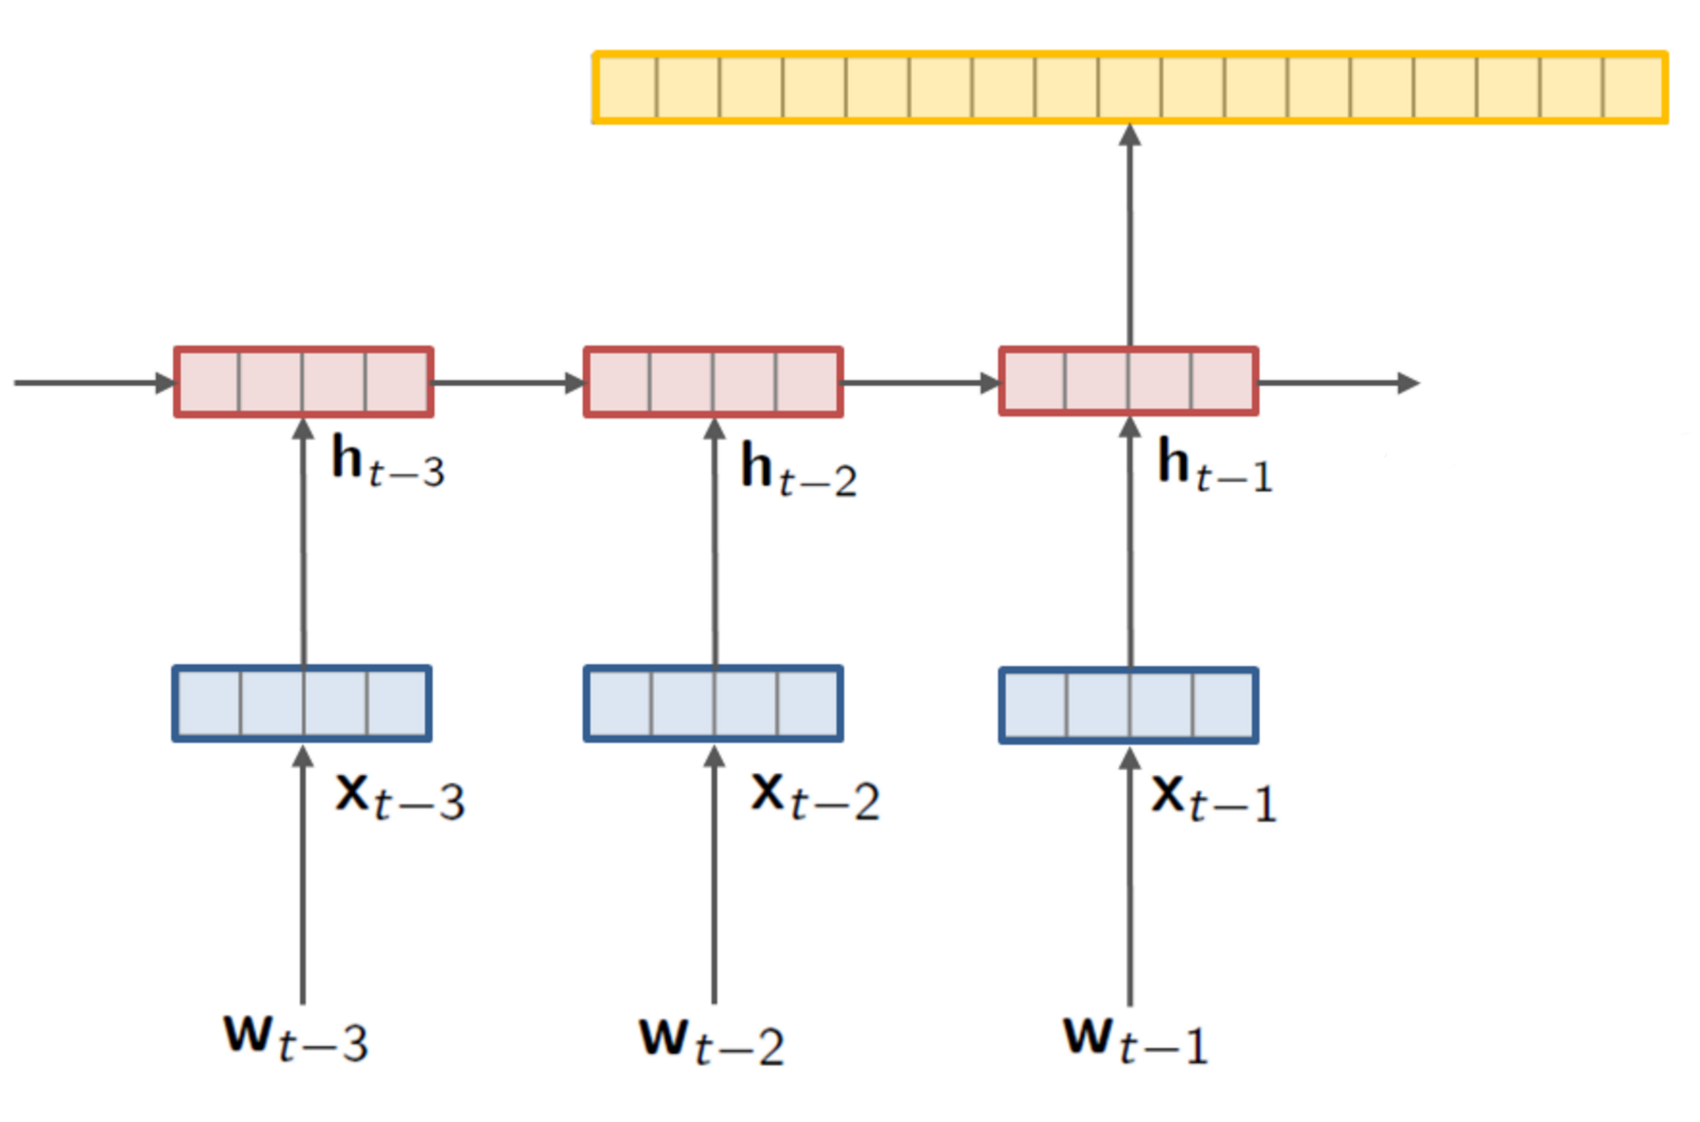
\includegraphics[width=0.6\textwidth]{rnnlm6}
    \end{center}
  \begin{itemize}
  \item Key idea, contextual language model based on encoder $x$: 
  \end{itemize}
  \[ p(w_{1:T} | x) = \prod_{t} p(w_t | w_1, \ldots, w_{t-1}, x) \] 
  
\end{frame}

\begin{frame}
  \begin{center}
    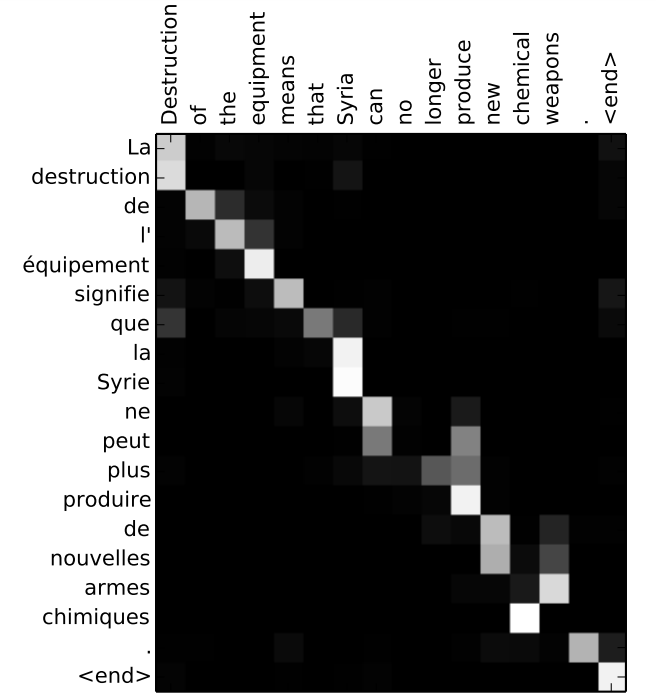
\includegraphics[width=0.6\textwidth]{attenalign}
  \end{center}
\end{frame}


\begin{frame}
  \begin{center}
    Actual Seq2Seq / Encoder-Decoder / Attention-Based Models
  \end{center}
    \begin{center}
      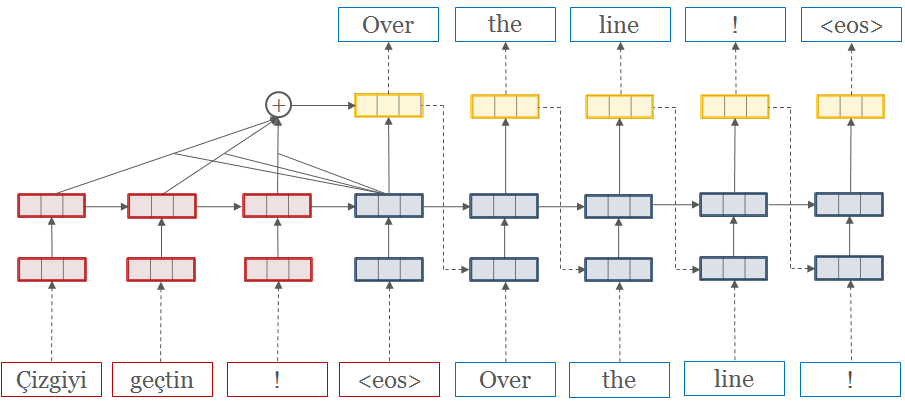
\includegraphics[width=0.7\textwidth]{simple-attn}
    \end{center}
  \begin{itemize}
  \item Different encoders, attention mechanisms, input feeding, ...
    \air
  \item Almost all models use LSTMs or other gated RNNs 
    \air
  \item Large multi-layer networks  necessary for good performance.
    \begin{itemize}
    \item 4 layer, 1000 hidden dims is common for MT
    \end{itemize}
  % \item Main idea, contextual language model based on encoder $\cvec$: 
  \end{itemize}
  % \[ p(w_{1:T} | \cvec) = \prod_{t} p(w_t | w_1, \ldots, w_{t-1}, \cvec) \] 
\end{frame}



\begin{frame}[fragile]
  \begin{center}
    \textbf{Beam Search} ($K = 3$)
  \end{center}
  \air 

    \begin{center}
  \begin{tikzpicture}[transform canvas = {scale=0.8}]
    \tikzstyle{beam}=[draw, minimum height=0.6cm, anchor=base, text height=5, text depth=0, minimum width=1.5cm,thin, rounded corners, line width=0.03cm]
   \tikzstyle{mat}=[draw=white]
    \tikzset{>=stealth',every on chain/.append style={join},
      every join/.style={->}}

     
       \begin{scope}
         
   \matrix (G) [matrix of nodes, nodes={beam},inner sep=1mm,row sep=0.03cm, column sep=0.8cm ] {
    \node<1->(G-1-1){a}; & \node<7->(G-1-2){red}; & \node<8->(G-1-3){dog}; & \node<9->(G-1-4){smells}; & \node<10->(G-1-5){home};  & \node<11->(G-1-6){today}; \\
    \node<1->(G-2-1){the}; & \node<7->(G-2-2){dog}; & \node<8->(G-2-3){dog}; & \node<9->(G-2-4){barks}; & \node<10->(G-2-5){quickly}; & \node<11->(G-2-6){Friday}; \\
    \node<1->(G-3-1){red}; & \node<7->(G-3-2){blue}; & \node<8->(G-3-3){cat}; &  \node<9->(G-3-4){walks}; & \node<10->(G-3-5){straight}; & \node<11->(G-3-6){now}; \\    };

    \only<7->{
      \draw[->] (G-1-1.east) -> (G-1-2.west); 
      \draw[->] (G-2-1.east) -> (G-2-2.west); 
      \draw[->] (G-1-1.east) -> (G-3-2.west); 
      \draw[double, line width=0.03cm] (G-3-1.south west) -- (G-3-2.south east);
    }
  
    \only<8->{
      \draw[->] (G-1-2.east) -> (G-2-3.west); 
      \draw[->] (G-3-2.east) -> (G-3-3.west); 
      \draw[->] (G-3-2.east) -> (G-1-3.west); 
      \draw[double, line width=0.03cm] (G-3-1.south west) -- (G-3-3.south east);
    }
    
 \only<9->{
    \draw[->] (G-1-3.east) -> (G-3-4.west); 
    \draw[->] (G-2-3.east) -> (G-2-4.west); 
    \draw[->] (G-1-3.east) -> (G-1-4.west); 
    \draw[double, line width=0.03cm] (G-3-1.south west) -- (G-3-4.south east);
}
 \only<11->{
    \draw[->] (G-1-5.east) -> (G-1-6.west); 
    \draw[->] (G-1-5.east) -> (G-3-6.west); 
    \draw[->] (G-2-5.east) -> (G-2-6.west); 
    \draw[double, line width=0.03cm] (G-3-1.south west) -- (G-3-6.south east);
}

 \only<10->{
    \draw[->] (G-3-4.east) -> (G-1-5.west); 
    \draw[->] (G-3-4.east) -> (G-2-5.west); 
    \draw[->] (G-3-4.east) -> (G-3-5.west); 
    \draw[double, line width=0.03cm] (G-3-1.south west) -- (G-3-5.south east);
}

\end{scope}
\end{tikzpicture}
\end{center}

    \air
    \air
    \air
For $t \niceq 1 \ldots T$:
   \begin{itemize}
   \item For all $k$ and for all possible output words $w$:
     \begin{align*}
     \alert<2>{s(w, \hat{y}_{1:t-1}^{(k)})} \gets \alert<3>{\log p(\hat{y}^{(k)}_{1:t-1}| x)} + \alert<4>{\log p(w | \hat{y}^{(k)}_{1:t-1}, x)} \end{align*}
   \item Update beam:
%     \begin{align*}
%     \hspace*{-4.4cm} \hat{y}_{1:t}^{(1:K)} \gets \topK_{s} \left\lbrace \mcV \times \hat{y}_{1:t-1}^{(1:K)} \right\rbrace
%\end{align*}  
\begin{align*}
\hspace*{-4cm} \alert<5>{\hat{y}_{1:t}^{(1:K)}} \gets \alert<6>{\kargmax} \, s(w, \hat{y}_{1:t-1}^{(k)})
\end{align*}
   \end{itemize}
\end{frame}


\begin{frame}
  \begin{center}

  \textbf{Applications}
\end{center}

\end{frame}

\begin{frame}
  \centerline{\textbf{Seq2Seq-Attn}   }

  \begin{itemize}
  \item HarvardNLP's open-source system (Yoon Kim) \href[pdfnewwindow=true]{http://github.com/harvardnlp/seq2seq-attn}{http://github.com/harvardnlp/seq2seq-attn}
    \air 
  \item Used by SYSTRAN for 32 language pairs \Cite{systran}
  \end{itemize}
  
  \begin{center}
    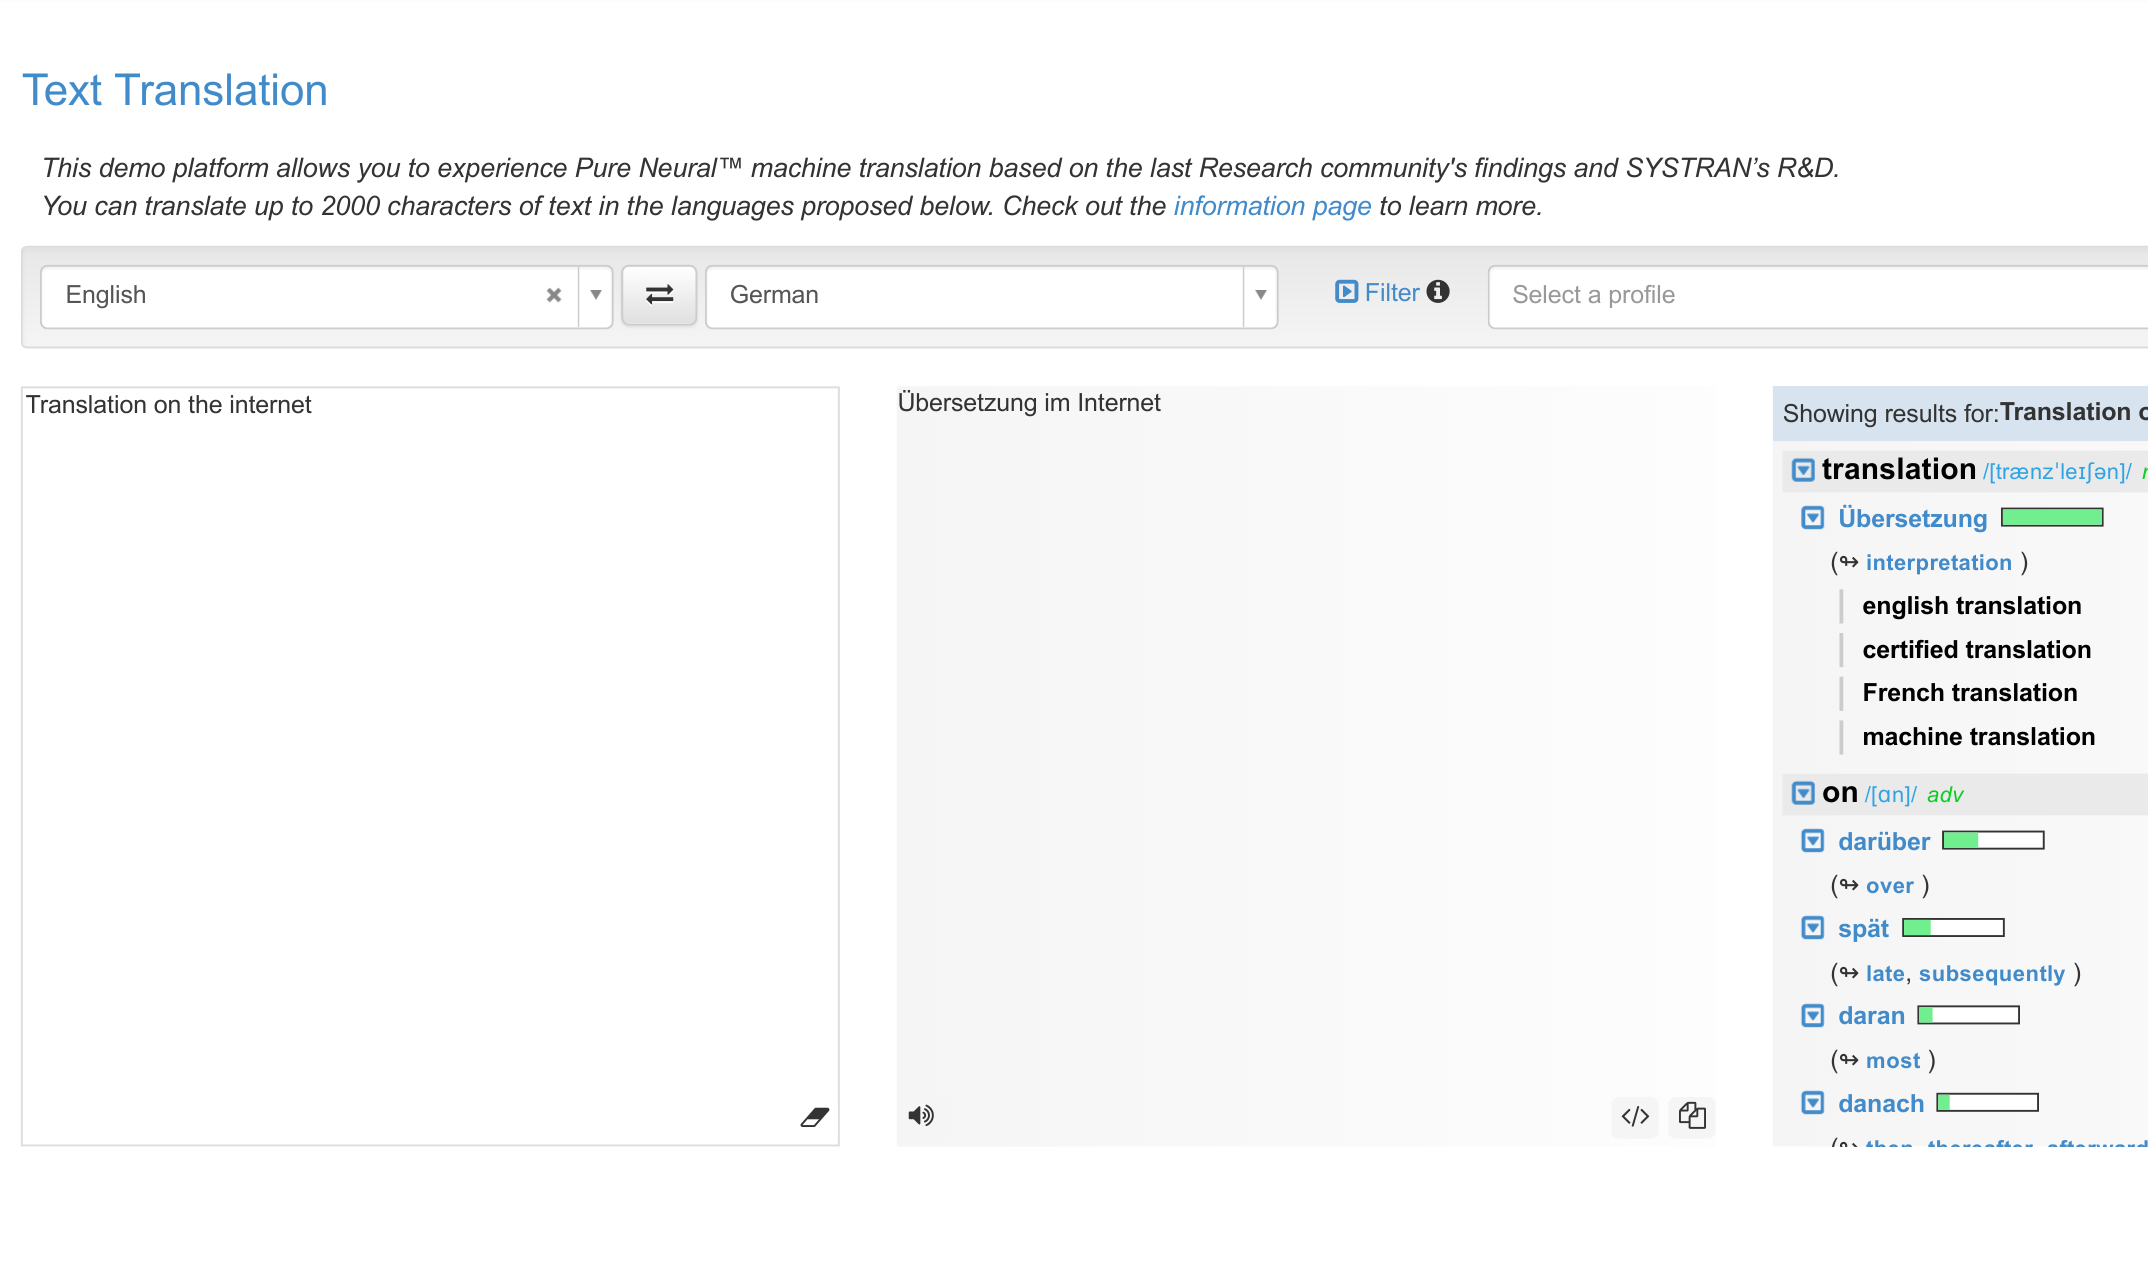
\includegraphics[width=0.9\textwidth]{systran}

    \href[pdfnewwindow=true]{http://demo-pnmt.systran.net}{[Demo]}
  \end{center}

\end{frame}


\begin{frame}
  \centerline{\textbf{Seq2Seq Applications:} \alert{Neural Summarization} \Cite{Rush2015} }
  \begin{center}
    \textbf{Source} (First Sentence)
  \end{center}
  
  \begin{figure}
    \textit{\structure<2>{Russian Defense Minister Ivanov}
      called \structure<2>{Sunday} for the creation of
      a joint front \structure<2>{for combating} global terrorism. }
  \end{figure}

  \begin{center}
    \textbf{Target} (Title)
  \end{center}
  \mair

  \begin{figure}
    \centering
    \textit{\alert<2>{Russia} calls for joint
      front \alert<2>{against} terrorism.}
  \end{figure}

\air
\air

  \begin{itemize}
  \item \Cite{mou2015backward} \Cite{cheng2016neural} \Cite{toutanovadataset} \Cite{wang2016experimental} \Cite{takaseneural}, among others
  \item Used by Washington Post to suggest headlines \Cite{shuguangwang}
  \end{itemize}
\end{frame}

\begin{frame}
  \centerline{\textbf{Seq2Seq Applications:} \alert{Grammar Correction} \Cite{Schmaltz2016} }
  % \centerline{\structure{Grammar Correction} \cite{}}
  
  \begin{center}
    \textbf{Source} (Original Sentence)
  \end{center}
  
  \begin{figure}
    \textit{There is no \structure{a doubt}, tracking \structure{systems has} brought many benefits in this information
age . }
  \end{figure}

  \begin{center}
    \textbf{Target} (Corrected Sentence)
  \end{center}
  \mair

  \begin{figure}
    \centering
    \textit{There is no doubt, tracking systems have
      brought many benefits in this information
      age . }
  \end{figure}

  \begin{itemize}
  \item 1st on BEA'11 grammar correction task \Cite{Daudaravicius2016}
  \end{itemize}
\end{frame}


\begin{frame}
  \centerline{\textbf{Seq2Seq Applications:} \alert{Im2Markup} (Deng and Rush, 2016) }
  
  \air 

  \begin{center}
    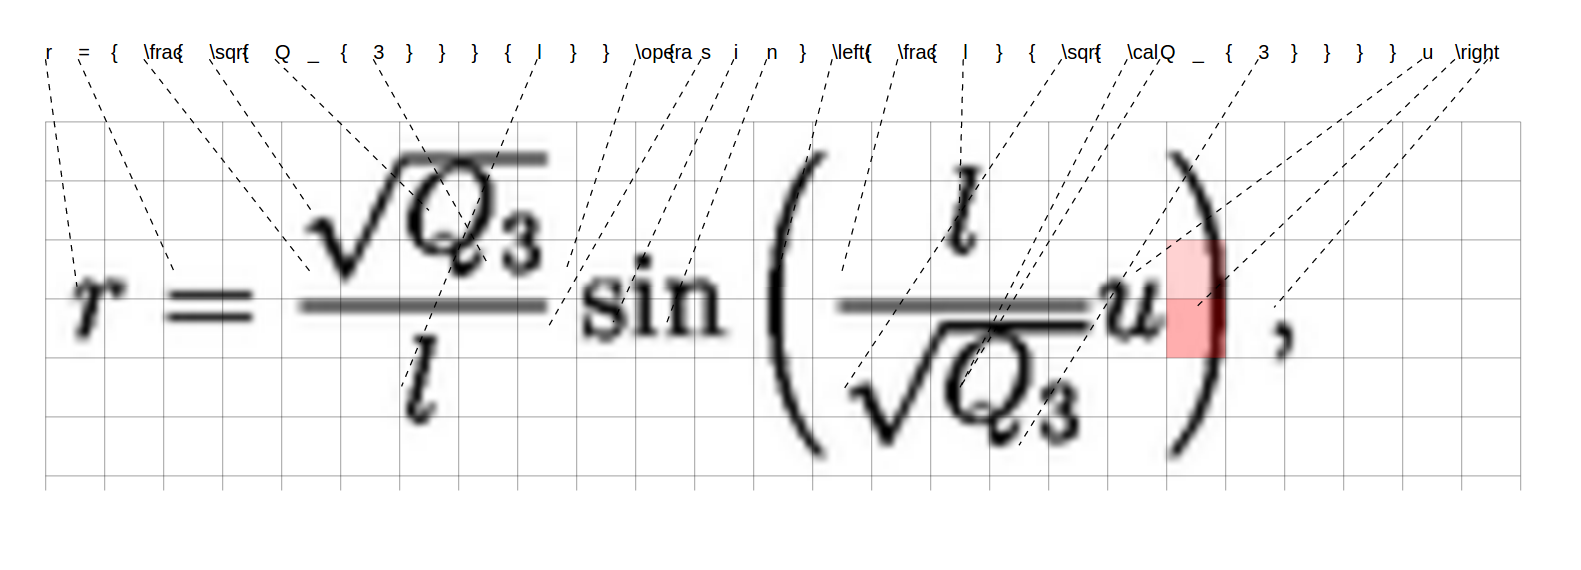
\includegraphics[width=\textwidth]{math}
  \end{center}
  % \movie[width=\textwidth, height=4cm, poster, repeat]{}{Latex.mp4}
  


  \begin{figure}
    \centering
  \end{figure}

  \centerline{\href[pdfnewwindow=true]{https://harvardnlp.github.io/seq2seq-talk/web/math.html}{[Latex Example]}}
  \centerline{\href[pdfnewwindow=true]{http://lstm.seas.harvard.edu/latex}{[Project]}}
\end{frame}


\begin{frame}{}
  \begin{center}
    \structure{Sequence-to-Sequence}
  \end{center}

  \begin{itemize}
  \item \alert<2>{Machine Translation} \Cite{kalchbrenner2013recurrent,sutskever2014sequence, Cho2014, bahdanau2014neural,luong15effective} 
    \air

   
  \item Question Answering \Cite{Hermann2015} 
  \item Conversation \Cite{Vinyals2015} \Cite{Serban2016}
  \item Parsing \Cite{vinyals15grammar}
  \item Speech \Cite{Chorowski2015,Chan2015}
  \item Caption Generation \Cite{karpathy2015deep,Xu2015,Vinyals2015b}
  \item Video-Generation \Cite{Srivastava2015a}
  \item NER/POS-Tagging \Cite{Gillick2016}
  \item Summarization \Cite{Rush2015} 
    \air 

  \end{itemize}  
\end{frame}


% \begin{frame}
%   \centerline{\textbf{Seq2Seq Details}}
%   \textbf{\structure{Train Objective}}: Given source-target pairs $(x, y_{1:T})$, minimize NLL of each word independently, conditioned on \textit{gold} history $y_{1:t-1}$
% \begin{align*}
% {\cal L}_{\text{NLL}}(\theta) = -\sum_{t} \log p(w_{t} = y_t | y_{1:t-1}, x; \theta) 
% \end{align*}

%   \air

% \textbf{\alert{Test Objective}}:  Structured prediction
%   \begin{align*}
%   \hat{y}_{1:T} = \argmax_{w_{1:T}} \sum_{t} \log p(w_{t} | w_{1:t-1}, x; \theta)
% \end{align*}
% \begin{itemize}
% \item Typical to approximate the $\argmax$ with beam-search
% \end{itemize}
% \end{frame}

% \begin{frame}
%   \begin{center}
%     \textbf{Interpreting RNNs}
%   \end{center}
% \end{frame}



% \begin{frame}
%   \centerline{\structure{This Talk}}
%   \air 
%   \air

%   \begin{itemize}
%   \item How can we \textbf{interpret} these learned hidden representations? 
%     \air 

    

%   \item  How should we \textbf{train} these style of models? 
%     \air 
%   \item  How can we \textbf{shrink} these models for practical applications? 
%   \end{itemize}
% \end{frame}


% \begin{frame}
%   \centerline{\structure{This Talk}}
%   \air 
%   \air

%   \begin{itemize}
%   \item How can we \textbf{interpret} these learned hidden representations? 

%     \begin{center}
%       \alert{LSTMVis}   
%       \href[pdfnewwindow=true]{https://lstm.seas.harvard.edu/}{lstm.seas.harvard.edu}

%       \Cite{Strobelt2016}

%       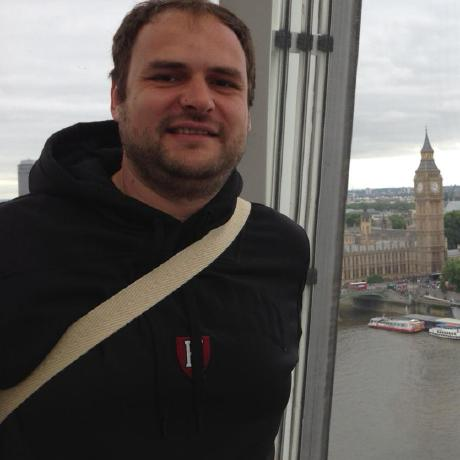
\includegraphics[width=2cm]{hen}
%     \end{center}


%     \air 

    

%   \item  \textcolor{gray}{How should we \textbf{train} these style of models? \Cite{Wiseman2016a}}
%     \air 
%   \item  \textcolor{gray}{How can we \textbf{shrink} these models for practical applications? \Cite{Kim2016a}}
%   \end{itemize}
% \end{frame}

\section{Interpretation}

\begin{frame}
  \begin{center}
    \textbf{Interpreting RNNs}
  \end{center}
\end{frame}


% \begin{frame}
%   \air 
%   \includegraphics[width=\textwidth,trim={0 0 0 19.5cm},clip]{filters}
%   \begin{center}
%      \Cite{DBLP:conf/eccv/ZeilerF14}
%   \end{center}
% \end{frame}

% \begin{frame}
%   \begin{frame}
%   \begin{center}
%     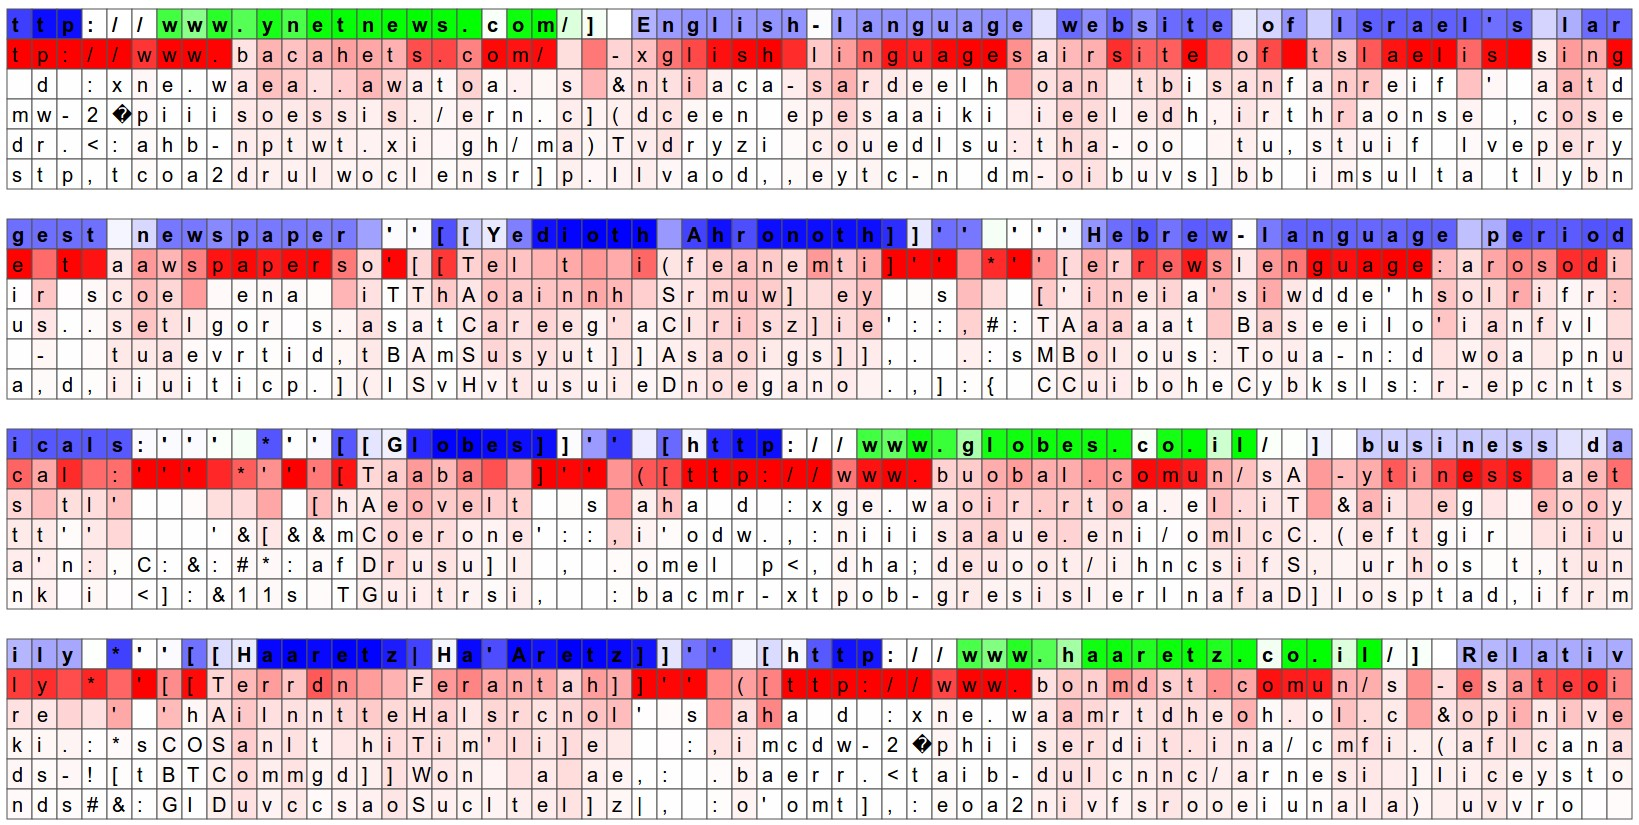
\includegraphics[width=\textwidth]{lstm1}

%     {\footnotesize (Karpathy et al, 2015)}
%   \end{center}

%     % \caption{Xu et al (2015)}  
% \end{frame}

\begin{frame}
  \air 
  \includegraphics[width=\textwidth,trim={0 0 0 19.5cm},clip]{filters}
  \begin{center}
     \Cite{DBLP:conf/eccv/ZeilerF14}
  \end{center}
\end{frame}


\begin{frame}
  % \begin{frame}
  \centerline{Vector-Space RNN Representation}
  \begin{center}
    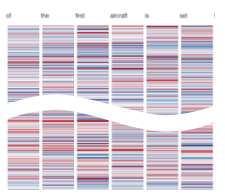
\includegraphics[height=5cm]{lstmrep}
  \begin{center}
    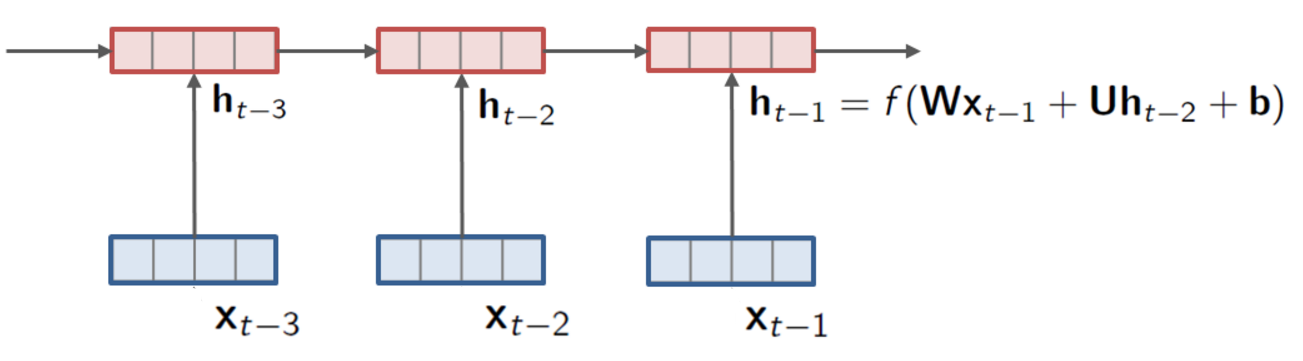
\includegraphics[width=11cm]{rnn}
  \end{center}
  \end{center}
\end{frame}


\begin{frame}
  % \begin{frame}
  \begin{center}
    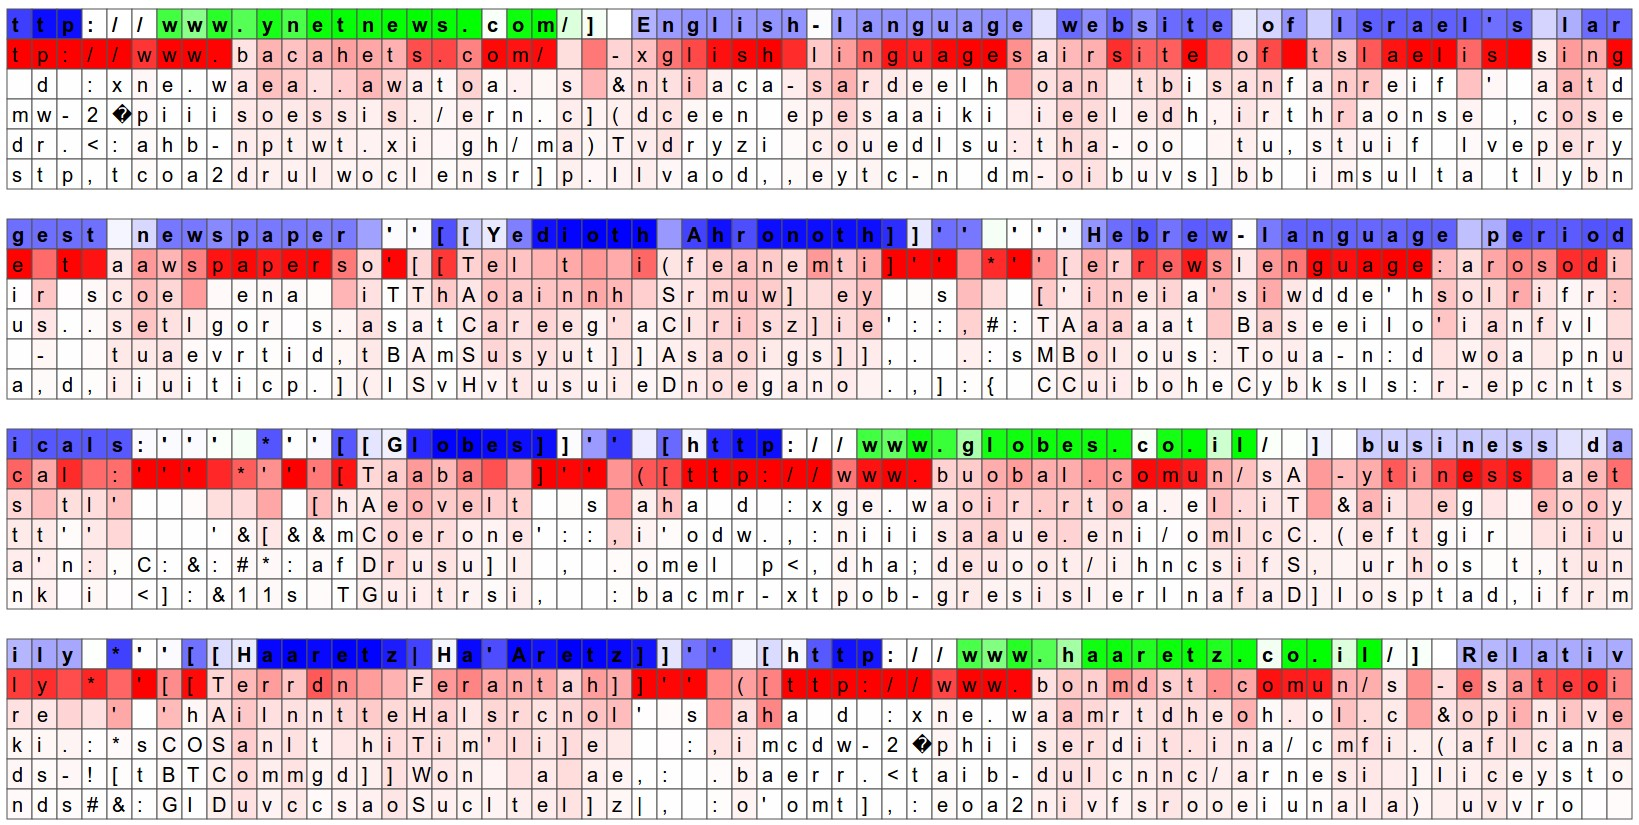
\includegraphics[width=\textwidth]{lstm1}
4
     \Cite{karpathy2015visualizing}
    % {\footnotesize (Karpathy et al, 2015)}
  \end{center}
    % \caption{Xu et al (2015)}  
\end{frame}

\begin{frame}
  \centerline{\alert{Example 1}: Synthetic (Finite-State) Language}
  \air

  \begin{center}
    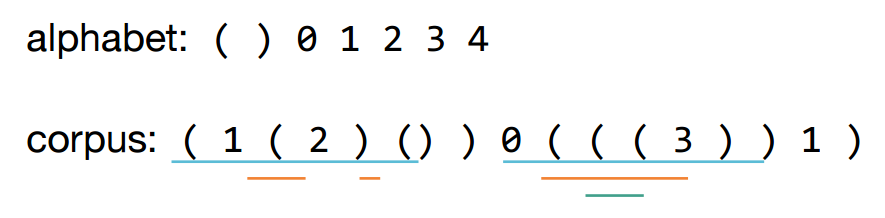
\includegraphics[width=9cm]{parenlang}
  \end{center}
  \mair

  \begin{itemize}
  \item Numbers are randomly generated, must match nesting level.
    \air

  \item Train a predict-next-word language model (decoder-only).
  \end{itemize}
    \[ p(w_t | w_1, \ldots, w_{t-1}) \] 
  
\air
  \centerline{\href[pdfnewwindow=true]{http://lstm.seas.harvard.edu/client/pattern_finder.html?data_set=00parens&source=states::states2&pos=150}{[Parens Example]}}
\end{frame}


\begin{frame}
  \centerline{\alert{Example 2}: Real Language}
  \air

  \begin{description}
  \item[alphabet:] all english words
  \item[corpus:] Project Gutenberg Children's books 
  \end{description}
  % \begin{center}
  %   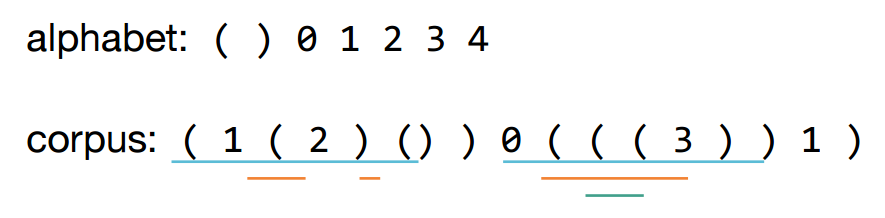
\includegraphics[width=9cm]{parenlang}
  % \end{center}

  \begin{itemize}
  % \item 
  %   \air

  \item Train a predict-next-word language model (decoder-only).

  
  \end{itemize}
    \[ p(w_t | w_1, \ldots, w_{t-1}) \] 

\air
  \centerline{ \href[pdfnewwindow=true]{http://lstm.seas.harvard.edu/client/pattern_finder.html?data_set=05childbook&source=states::states1&pos=100}{[LM Example]}}
\end{frame}


\begin{frame}
  \centerline{\alert{Example 3}: Seq2Seq Encoder}
  \air

  \begin{description}
  \item[alphabet:] all english words
  \item[corpus:]  Summarization
  \end{description}
  % \begin{center}
  %   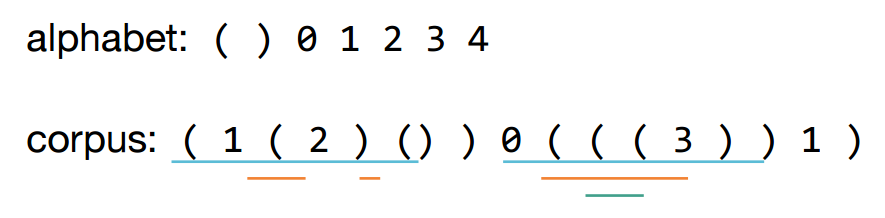
\includegraphics[width=9cm]{parenlang}
  % \end{center}

  \begin{itemize}
  % \item 
  %   \air

  \item Train a full seq2seq model, examine \textit{encoder} LSTM.
  
  \end{itemize}


\air
  \centerline{ \href[pdfnewwindow=true]{http://lstm.seas.harvard.edu/client/pattern_finder.html?data_set=20autoencoder&source=states::states2&pos=100}{[Summarization Example]}}
\end{frame}
% \begin{frame}
%   \centerline{\structure{This Talk}}
%   \air 
%   \air

%   \begin{itemize}
%   \item \textcolor{gray}{How can we \textbf{interpret} these learned hidden representations? \Cite{Strobelt2016}}
%     \air 
%   \item  How should we \textbf{train} these style of models? 
%     \air 

%     \begin{center}
%       \alert{Sequence-to-Sequence Learning as Beam-Search
%         Optimization}
     
%       \Cite{Wiseman2016a}

%       
\includegraphics[width=2cm]{sam}
%     \end{center}


%     \air 
%   \item \textcolor{gray}{ How can we \textbf{shrink} these models for practical applications \Cite{Kim2016a}? }
%   \end{itemize}
% \end{frame}


\begin{frame}
  \begin{center}
    \textbf{Future Work}
  \end{center}

  \begin{center}

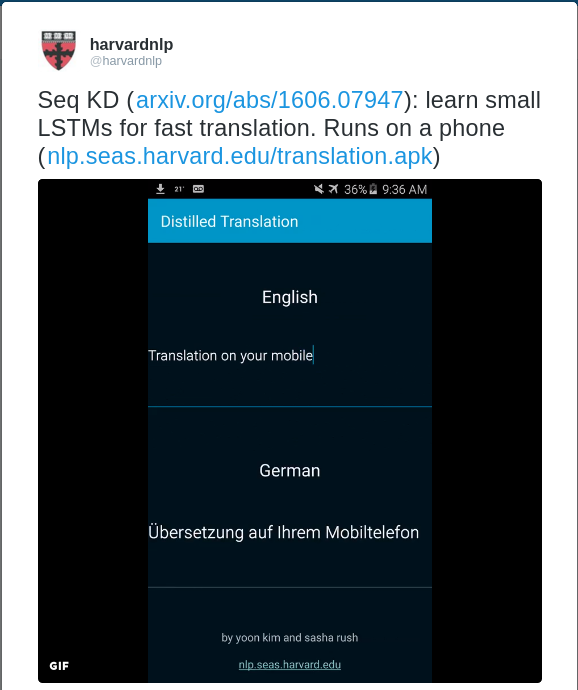
\includegraphics[width=5cm]{phonemt}
  \end{center}

  \href[pdfnewwindow=true]{https://harvardnlp.github.io/seq2seq-talk/transfast.gif}{[App]}

\end{frame}

\begin{frame}
\begin{center}
Thanks!
\end{center}
\end{frame}


% \begin{frame}
%   \begin{center} 
%     \structure{Thank You}
%   \end{center}
%   \air 
%   \begin{center}
%     
\includegraphics[width=3cm]{harvardnlp}
%   \end{center}
%   % \structure{Focus:} Deep learning of the representation of language structure

%   \begin{center}
%     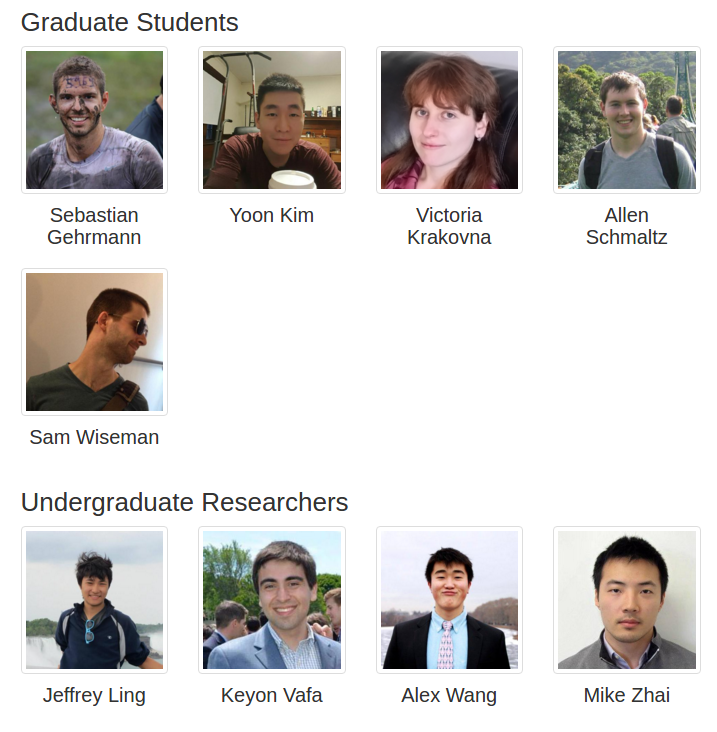
\includegraphics[width=6cm]{harvardnlpgroup}
%   \end{center}
  
% \end{frame}



\begin{frame}[t,allowframebreaks]
  \frametitle{References}
  \begin{small}
    \bibliography{full,career2,seq2seqapps,ourwork,master,masterseqk,beamtrain}
  \end{small}
 \end{frame}

\bibliographystyle{apalike}

\end{document}
